% \documentclass[11pt,table,final,fleqn,xcolor={usenames,dvipsnames},unknownkeysallowed,handout]{beamer}
% \usetheme[]{Frankfurt}
% \usecolortheme{crane}

% % \usepackage{listings}
% % \usepackage{multimedia} % Movies
% % \usepackage{fancyvrb,relsize}
% % \usepackage{commath}
% % \usepackage{graphicx}
% % \usepackage{longtable}
% % \usepackage[math]{iwona}
% % \usepackage{wasysym}
% % \usepackage{amsmath} 
% % \usepackage{amssymb}
% % \usepackage[amssymb]{SIunits}
% % \usepackage{tikz} % Drawing

% 
\usepackage{listings}
\usepackage{multimedia} % Movies
\usepackage{fancyvrb,relsize}
\usepackage{commath}
\usepackage{graphicx}
\usepackage{array}
\usepackage{longtable}
\usepackage{algpseudocode} 
\usepackage{multirow}
\usepackage[math]{iwona}
\usepackage{wasysym}
% \usepackage[fleqn]{amsmath}
\usepackage{amssymb}
\usepackage{siunitx}
\usepackage{tikz} % Drawing
\usepackage{pgfplots}
\usepackage{pgfplotstable}
% \usepackage{fontspec}

% Presentation settings
\rowcolors[]{1}{maincolor!20}{maincolor!10}

\newcommand{\Fo}{\ensuremath{\mathit{Fo}}}

\lstset{language=Matlab,%
    %basicstyle=\color{red},
    basicstyle=\scriptsize\ttfamily,
    breaklines=true,%
    morekeywords={matlab2tikz},
    keywordstyle=\color{blue},%
    morekeywords=[2]{1}, keywordstyle=[2]{\color{black}},
    identifierstyle=\color{black},%
    stringstyle=\color{mylilas},
    commentstyle=\color{mygreen},%
    showstringspaces=false,%without this there will be a symbol in the places where there is a space
    numbers=none,%
%     numberstyle={\tiny \color{black}},% size of the numbers
%     numbersep=-2pt, % this defines how far the numbers are from the text
%     emph=[1]{for,end,break},emphstyle=[1]\color{red}, %some words to emphasise
emph=[2]{ones,int,str2double,long,single,simplify,diff,log,atan,solve,vpa,syms,doc,int,simplify,diff,log,atan,syms,interp3,interpn,histogram,ribbon,contourf,fzero,feval,fminsearch,fsolve,fminbnd,ezplot,varargin,optimset,odeset,ode15s,plotyy,ones,linprog,cftool,optimset,lsqnonlin}, emphstyle=[2]{\color{blue}},
    backgroundcolor=\color{gray!15},frame=tlbr, framerule=0pt,
    escapeinside={(*@}{@*)}
}

% To have the navigation circles without declaring subsections
\usepackage{remreset}% tiny package containing just the \@removefromreset command
\makeatletter
\@removefromreset{subsection}{section}
\makeatother
\setcounter{subsection}{1}

% For convenient figure inclusion
\DeclareGraphicsExtensions{.pdf,.png,.jpg}
\graphicspath{ {../img/} }


% \setmainfont{Yanone Kaffeesatz}
% \setmathfont(Digits,Latin,Greek)[Numbers={Lining,Proportional}]{Gentium Plus}

% TU/e colors
\definecolor{tuered}{RGB}{247,49,49}
\definecolor{tuefuchsia}{RGB}{214,0,74}
\definecolor{tuelila}{RGB}{214,0,123}
\definecolor{tuepurple}{RGB}{173,32,173}
\definecolor{tuedblue}{RGB}{16,16,115}
\definecolor{tueblue}{RGB}{0,102,204}
\definecolor{tuelblue}{RGB}{0,162,222}
\definecolor{tueorange}{RGB}{255,154,0}
\definecolor{tueyellow}{RGB}{255,221,0}
\definecolor{tuedyellow}{RGB}{206,223,0}
\definecolor{tuegreen}{RGB}{132,210,0}
\definecolor{tuedgreen}{RGB}{0,172,130}
\definecolor{tueblue2}{RGB}{0,146,181}

% For Matlab script colors
\definecolor{mygreen}{RGB}{28,172,0} % color values Red, Green, Blue
\definecolor{mylilas}{RGB}{170,55,241}

\makeatletter
% \definecolor{beamer@blendedblue}{rgb}{0.5,0.5,0.3} % changed this
\useoutertheme{smoothbars}
\useinnertheme{circles}

%%%%%%%%%%%%%%%%%%%%%%%%%%%%%%%%%%%%%%%%%%%%%%%%%%%%%%%%%%%%%%%%%%%%%%%%%%%
\definecolor{maincolor}{named}{tuelblue}
\definecolor{textcolorfg}{named}{white}
\definecolor{tuealert}{named}{tueblue}
%%%%%%%%%%%%%%%%%%%%%%%%%%%%%%%%%%%%%%%%%%%%%%%%%%%%%%%%%%%%%%%%%%%%%%%%%%%

\setbeamercolor{normal text}{fg=black,bg=white}
\setbeamercolor{alerted text}{fg=tuealert}
\setbeamercolor{example text}{fg=tuegreen!50!black}

\setbeamercolor{background canvas}{parent=normal text,bg=white}
\setbeamercolor{background}{parent=background canvas}

\setbeamercolor{title}{bg=maincolor,fg=textcolorfg} % Presentation title colors
\setbeamercolor{structure}{fg=maincolor,bg=textcolorfg}
\setbeamercolor{section in head/foot}{fg=textcolorfg,bg=maincolor}
\setbeamercolor{palette primary}{fg=textcolorfg,bg=maincolor} % changed this

\setbeamercolor{palette primary}{fg=maincolor,bg=textcolorfg} % changed this
\setbeamercolor{palette secondary}{use=structure,fg=structure.fg!100!tueblue} % changed this
\setbeamercolor{palette tertiary}{use=structure,fg=structure.fg!100!tuered} % changed this

\setbeamertemplate{navigation symbols}{} % ( Dont use )
\setbeamercolor{navigation symbols}{use=structure,fg=structure.fg!40!bg}
\setbeamercolor{navigation symbols dimmed}{use=structure,fg=structure.fg!20!bg}

\setbeamercolor{block title}{fg=textcolorfg,bg=maincolor}
\setbeamercolor{block body}{fg=black,bg=maincolor!10}

\def\colorize<#1>{%
  \temporal<#1>{\color{tuedblue!40!gray!40}}{\color{tuealert}}{\color{black}}}
  
\setlength{\mathindent}{0pt}

\makeatother

% Colored urls
\hypersetup{colorlinks,linkcolor=,urlcolor=tueblue}

% Vector format
\renewcommand{\vec}[1]{\mathbf{#1}}

\usetikzlibrary{decorations} % Drawing
\usetikzlibrary{patterns}
\usetikzlibrary{positioning}
\usetikzlibrary{shadows}
\usetikzlibrary{calc}
\usetikzlibrary{arrows}
\usetikzlibrary{decorations}
\usetikzlibrary{plotmarks}
\usetikzlibrary{shapes}
\usetikzlibrary{shadings}
\usetikzlibrary{intersections}
% Blocks
\tikzset{block/.style={rectangle,draw=maincolor,fill=maincolor!20,text width=10em,text centered,rounded corners,minimum height=4em,thick}}
\tikzset{emphblock/.style={rectangle,draw=maincolor,text centered,rounded corners,thick,top color=maincolor!10,bottom color=maincolor!30}}
% Dots
\tikzset{dot/.style={draw=tuered,circle,thick,minimum size=1mm,inner sep=0pt,outer sep=0pt,fill=white}}
\tikzset{fdot/.style={circle,draw=black,fill=black,,inner sep=1.5pt}}
\tikzset{gdot/.style={circle,draw=black,inner sep=3pt}}
\tikzset{cross/.style={cross out, draw=black, fill=none, minimum size=2*(#1-\pgflinewidth), inner sep=0pt, outer sep=0pt}, cross/.default={4pt}}
% Graphs and lines
\tikzset{line/.style={black,>=stealth',semithick}}
\tikzset{graph/.style={smooth,samples=400,tuered,semithick}}
\tikzset{interp/.style={dot,draw=tuealert,inner sep=1.5pt,minimum size=4pt,color=tuealert,fill=none}}
\tikzset{intblock/.style={line,draw=tuefuchsia,fill=tuefuchsia!50!white,fill opacity=0.3,opacity=0.6}}
\tikzset{intdot/.style={line,dot,draw=tuefuchsia,fill=tuefuchsia,opacity=0.6}}
\tikzset{gridline/.style={lightgray,ultra thin,dashed}}


\newcolumntype{L}[1]{>{\raggedright\arraybackslash}p{#1}}
\newcolumntype{R}[1]{>{\raggedleft\arraybackslash}p{#1}}

% \pgfplotsset{
% % every axis y label/.append style={at={axis cs:14,14},rotate=0,anchor=south east}
% exery axis/.style={ylabel near ticks},
% }


\renewcommand*\familydefault{\sfdefault}  % Use sans font
% % 
% % \usepackage{pgfpages}
% % \pgfpagesuselayout{4 on 1}[border shrink=5mm]

% % PRESENTATION SPECIFICS
% \title{Matlab and Programming 2}
% \subtitle{Advanced programming techniques}

% \author[I.~Roghair]{\underline{Ivo~Roghair}, Martin van Sint Annaland}

% \institute{Chemical Process Intensification\\Eindhoven University of Technology}

% \date

% % BEGIN PRESENTATION
% \begin{document}
% \lstset{language=Matlab,%
    %basicstyle=\color{red},
    basicstyle=\footnotesize\ttfamily,
    breaklines=true,%
    morekeywords={matlab2tikz},
    keywordstyle=\color{blue},%
    morekeywords=[2]{1}, keywordstyle=[2]{\color{black}},
    identifierstyle=\color{black},%
    stringstyle=\color{mylilas},
    commentstyle=\color{mygreen},%
    showstringspaces=false,%without this there will be a symbol in the places where there is a space
    numbers=none,%
%     numberstyle={\tiny \color{black}},% size of the numbers
%     numbersep=-2pt, % this defines how far the numbers are from the text
%     emph=[1]{for,end,break},emphstyle=[1]\color{red}, %some words to emphasise
    emph=[2]{ones,int,simplify,diff,log,atan,syms,doc,int,simplify,diff,log,atan,syms,interp3,interpn,histogram,ribbon,contourf,fzero,feval,fminsearch,fsolve,fminbnd,ezplot,varargin,optimset,odeset,plotyy,ones,linprog,cftool,optimset,lsqnonlin}, emphstyle=[2]{\color{blue}},
    backgroundcolor=\color{gray!15},frame=tlbr, framerule=0pt,
    escapeinside={(*@}{@*)}
}

% \frame[plain]{
%   \titlepage
% }

\section{Coding in style}
\subsection*{Introduction}
\begin{frame}[label=contents]
  \frametitle{Today's outline}
  \mode<beamer>{
    \only<1>{\tableofcontents}
  }
  \only<2>{\tableofcontents[currentsection]}
\end{frame}

\begin{frame}
  \frametitle{If anything sticks today, let it be this}
  \begin{center}
    {\LARGE Your code will not be understood by anyone\\}
  \pause
  \vskip1em
  That includes future-you
  \vskip2em
  \end{center}
\end{frame}

\subsection*{Organization}
\begin{frame}
\frametitle{Code organization}
  \begin{itemize}
    \item Optimization of a code is time-consuming and complicated
    \item The more you optimize your code, the less readable it becomes
    \item But... You can write it in a such way that it will be flexible and easy to maintain
    \item Especially important in team work
    \item Any person has its own handwriting. Any programmer has its own coding style.
\end{itemize}
 \tikz{\node[emphblock,text width=\textwidth]{The coding style $\equiv$ handwriting...};}

\end{frame}

\begin{frame}[fragile]
 \frametitle{Interpret the following code}
 \begin{lstlisting}
s=checksc();
if(s==true)
a=cb();
b=cfrsp();
if(a<5)
if(b>5)
a=gtbs();
end
if(a>b)
ubx();
end
end
else
brn();
gtbs();
end
 \end{lstlisting}
\end{frame}

\begin{frame}[plain]

\includegraphics[keepaspectratio=true,width=\textwidth]{wat-2.jpg}
\end{frame}

\begin{frame}[fragile]
 \frametitle{Let's change that a bit... Indentation}
 \pause
 Shown here with 2 spaces of indentation, Matlab uses 4 by default!
 \begin{columns}[T]
    \column{0.4\textwidth}
     \begin{lstlisting}
s=checksc();
if(s==true)
a=cb();
b=cfrsp();
if(a<5)
if(b>5)
a=gtbs();
end
if(a>b)
ubx();
end
end
else
brn();
gtbs();
end
 \end{lstlisting}
    \column{0.6\textwidth}
     \begin{lstlisting}
s = checksc();
if (s == true)
  a = cb();
  b = cfrsp();
  if (a < 5)
    if (b > 5)
      a = gtbs();
    end
    if (a > b)
      ubx();
    end
  end
else
  brn();
  gtbs();
end
 \end{lstlisting}
 \end{columns}
\end{frame}

\begin{frame}[fragile]
 \frametitle{Readable variables and function names}
 \begin{columns}[T]
    \column{0.4\textwidth}
\begin{lstlisting}
s = checksc();
if (s == true)
  a = cb();
  b = cfrsp();
  if (a < 5)
    if (b > 5)
      a = gtbs();
    end
    if (a > b)
      ubx();
    end
  end
else
    brn();
    gtbs();
end
 \end{lstlisting}
    \column{0.6\textwidth}
     \begin{lstlisting}
IAmFree = checkSchedule();
if (IAmFree == true)
  books = countBooks();
  shelfSize = countFreeSpaceShelf();
  if (books < 5)
    if (shelfSize > 5)
      books = goToBookStore();
    end
    if (books > shelfSize)
      useBox();
    end
  end
else
  burnBooks();
  goToBookStore();
end
 \end{lstlisting}
 \end{columns}
%  \pause
%  \begin{itemize}
%   \item This style uses lowerCamelCase naming style. This is a personal preference.
%   \item Function names start with a verb; it \emph{does} something.
%  \end{itemize}
\end{frame}

\begin{frame}[fragile]
 \frametitle{Get rid of obscure constants in the code}
 \begin{columns}[T]
    \column{0.5\textwidth}
     \begin{lstlisting}[basicstyle=\scriptsize\ttfamily]
IAmFree = checkSchedule();
if (IAmFree == true)
  books = countBooks();
  shelfSize = countFreeSpaceShelf();
  if (books < 5)
    if (shelfSize > 5)
      books = goToBookStore();
    end
    if (books > shelfSize)
      useBox();
    end
  end
else
  burnBooks();
  goToBookStore();
end
 \end{lstlisting}
    \column{0.5\textwidth}
     \begin{lstlisting}[basicstyle=\scriptsize\ttfamily,emph={minBooksNeeded,maxShelfSize},emphstyle=\color{red}]
IAmFree = checkSchedule();
if (IAmFree == true)
  books = countBooks();
  shelfSize = countFreeSpaceShelf();
  if (books < maxShelfSize)
    if (shelfSize > minBooksNeeded)
      books = goToBookStore();
    end
    if (books > shelfSize)
      useBox();
    end
  end
else
  burnBooks();
  goToBookStore();
end
 \end{lstlisting}
 \end{columns}
\end{frame}

\begin{frame}[fragile]
 \frametitle{That's more like it!}
 \begin{columns}[T]
    \column{0.3\textwidth}
     \begin{lstlisting}
s=checksc();
if(s==true)
a=cb();
b=cfrsp();
if(a<5)
if(b>5)
a=gtbs();
end
if(a>b)
ubx();
end
end
else
brn();
gtbs();
end
 \end{lstlisting}
    \column{0.7\textwidth}
     \begin{lstlisting}
IAmFree = checkSchedule();
if (IAmFree == true)
  books = countBooks();
  shelfSize = countFreeSpaceShelf();
  if (books < maxShelfSize)
    if (shelfSize > minBooksNeeded)
      books = goToBookStore();
    end
    if (books > shelfSize)
      useBox();
    end
  end
else
  burnBooks();
  goToBookStore();
end
 \end{lstlisting}
 \end{columns}
\end{frame}

\subsection*{Comments}
\begin{frame}
  \frametitle{Writing readable code}
  Good code reads like a book.\vskip2em \pause
  \begin{itemize}
    \item When it doesn't, make sure to use comments. In Matlab, everything following \lstinline$ \% is a comment$
    \item Prevent ``smart constructions'' in the code
    \item Re-use working code (i.e. create functions for well-defined tasks).
    \item Documentation is also useful, but hard to maintain.\pause\ (Matlab comes with a function that generates reports from comments)
  \end{itemize}
\end{frame}

\begin{frame}[fragile]
 \frametitle{How not to comment}
 \begin{itemize}[<+->]
  \item Useless:
  \begin{lstlisting}
% Start program 
  \end{lstlisting}
  \item Obvious:
  \begin{lstlisting}
if (a > 5)   % Check if a is greater than 5
    ... 
end
else         % else add 1 to b
    b = b + 1;
end
  \end{lstlisting}
  \item Too much about the life:
  \begin{lstlisting}[basicstyle=\tiny\ttfamily]
% Well... I do not know how to explain what is going on
% in the snippet below. I tried to code in the night 
% with some booze and it worked then, but now I have a 
% strong hangover and some parameters still need to be
% worked out...
  \end{lstlisting}
 \end{itemize}
\end{frame}

\begin{frame}[fragile]
 \frametitle{Adding comments to our program}
 \begin{lstlisting}
IAmFree = checkSchedule();
if (IAmFree == true)
% Count books and amount of free space on a shelf. 
% If minimum number of books I need is less than a 
% shelf capacity, go shopping and buy additional 
% literature. If the amount of books after the 
% shopping is too big, use boxes to store them.
  books = countBooks();
  shelfSize = countFreeSpaceShelf();
  
  ...

else
  burnBooks();
  goToBookStore();
end
 \end{lstlisting}
\end{frame}

\begin{frame}
  \frametitle{If anything sticks today, let it be this}
  \begin{center}
    {\LARGE Your code will not be understood by anyone\\}
  \pause
  \vskip1em
  That includes future-you
  \vskip2em
  \end{center}
  \pause
  \tikz{\node[emphblock, text width=\textwidth]{Use comments and code to document design and purpose (functionality), not mechanics (implementation).};}
  \vskip1em\pause
  \tikz{\node[emphblock, text width=\textwidth]{Use consistent and sensible naming of functions and variables.};}
\end{frame}

\section{Error management}
\subsection*{Errors in programming}
\againframe<2>{contents}
\begin{frame}
 \frametitle{Errors in computer programs}
 \begin{center}
    Computer programs often contain errors (bugs): buildings collapse, governments fall, kittens will die.\\
      \vskip1em
    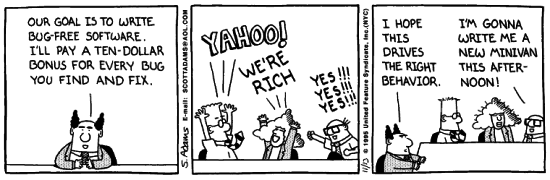
\includegraphics[width=0.8\textwidth]{bugFree.png}
 \end{center}
\end{frame}

\begin{frame}
 \frametitle{Errors in computer programs}
 \footnotesize\selectfont
 The following symptoms can be distinguished:
 \begin{itemize}
   \item Unable to execute the program
   \item Program crashes, warnings or error messages
   \item Never-ending loops
   \item Wrong (unexpected) result
 \end{itemize}
 \vskip1em
 \uncover<2->{
  Three error categories:
  \begin{description}
   \colorize<2->  \item[Syntax errors] You did not obey the language rules. These errors prevent running or compilation of the program.
   \colorize<3->  \item[Runtime errors] Something goes wrong during the execution of the program resulting in an error message (problem with input, division by zero, loading of non-existent files, memory problems, etc.)
   \colorize<4->  \item[Semantic errors] The program does not do what you expect, but does what have told it to do.
  \end{description}
 }
\end{frame}

% \begin{frame}[fragile]
%  \frametitle{Verification and validation}
%   \scriptsize\selectfont
%   \begin{columns}
%     \column{0.6\textwidth}
%     \uncover<3->{\begin{block}{Verification}
%     Verification is the process of mathematically and computationally assuring that the model computes what you have entered.    
%     \end{block}
%     }
%     \uncover<7->{
%     \begin{block}{Validation}
%       Validation is the process of determining the degree to which a model is an accurate representation of the real world from the perspective of the intended uses of the model
%     \end{block}
%     }
% 
%   \column{0.4\textwidth}
%     \begin{tikzpicture}[block/.style={rectangle,minimum size=3mm,text badly centered,drop shadow,
% 					thick,rounded corners,draw=maincolor,top color=maincolor!35,bottom color=maincolor!20,
% 					font=\sffamily\scriptsize},>=stealth,node distance=0.75cm]
% 	\node[block] (p) at (0,0) {Problem};
% 	\uncover<2->{\node[below of=p] (p1) {};
% 	\node[block, below of=p1] (mm) {Mathematical Model};
% 	\node[below of=mm] (mm1) {};}
% 	\uncover<4->{\node[block, below of=mm1] (cm) {Computational Model};
% 	\node[below of=cm] (cm1) {};}
% 	\uncover<6->{\node[block, below of=cm1] (r) {Results};}
% 	
% 	\uncover<3->{\node[block, left of=p1,node distance=2cm] (v1) {Verification};}
% 	\uncover<5->{\node[block, left of=mm1,node distance=2cm] (v2) {Verification};}
% 	\uncover<7->{\node[block, left of=cm1,node distance=2cm] (v3) {Validation};}
% 	
% 	\uncover<2->{\draw[->] (p) -> (mm);}
% 	\uncover<4->{\draw[->] (mm) -> (cm);}
% 	\uncover<6->{\draw[->] (cm) -> (r);}
% 	
% 	\uncover<3->{\draw[->] (v1) -> (p1);}
% 	\uncover<5->{\draw[->] (v2) -> (mm1);}
% 	\uncover<7->{\draw[->] (v3) -> (cm1);}
%     \end{tikzpicture}
%   \end{columns}
% 
% \end{frame}
% % 
% 
% \begin{frame}
%   \frametitle{Be aware of your uncertainties}
%   \scriptsize\selectfont
%   \begin{columns}
%     \column{0.5\textwidth}
%     \begin{center}
%       \mode<beamer>{
% 	\includegraphics<1>[width=0.8\columnwidth]{ptolemy1-1}
% 	\includegraphics<2>[width=0.8\columnwidth]{ptolemy1-2}
% 	\includegraphics<3>[width=0.8\columnwidth]{ptolemy1-3}
% 	\includegraphics<4>[width=0.8\columnwidth]{ptolemy1-4}
% 	\includegraphics<5>[width=0.8\columnwidth]{ptolemy1-5}
% 	\includegraphics<6>[width=0.8\columnwidth]{ptolemy1-6}
%       }
%       \includegraphics<7->[width=0.8\columnwidth]{ptolemy1-7}
%     \end{center}
%     \column{0.5\textwidth}
%     \begin{center}
%       \mode<beamer>{
% 	\includegraphics<7>[width=0.8\columnwidth]{ptolemy2-0}
% 	\includegraphics<8>[width=0.8\columnwidth]{ptolemy2-1}
% 	\includegraphics<9>[width=0.8\columnwidth]{ptolemy2-2}
% 	\includegraphics<10>[width=0.8\columnwidth]{ptolemy2-3}
% 	\includegraphics<11>[width=0.8\columnwidth]{ptolemy2-4}
% 	\includegraphics<12>[width=0.8\columnwidth]{ptolemy2-5}
% 	\includegraphics<13>[width=0.8\columnwidth]{ptolemy2-6}
%       }
%       \includegraphics<14>[width=0.8\columnwidth]{ptolemy2-7}
%     \end{center}
%   \end{columns}
%   \begin{itemize}
%     \item<7-> The perceived orbit of Mars from Earth shows a zig-zag (in contrast to the Sun, Mercury, Venus)
%     \item<14> Even though they were not 'right', Earth-centered models (Ptolemy) were still valid
%   \end{itemize}
% \end{frame}
% 
% \begin{frame}
%   \frametitle{Be aware of your uncertainties}
%   \vfill
%   \begin{block}{Aleatory uncertainty}
%     Uncertainty that arises due to inherent randomness of the system, features that are too complex to measure and take into account
%   \end{block}
%   \vskip1em
%   \begin{block}{Epistemic uncertainty}
%       Uncertainty that arises due to lack of knowledge of the system, but could in principle be known
%   \end{block}
%   \vfill
% \end{frame}

%  
\subsection*{Debugging}
\begin{frame}
\frametitle{A convenient tool: the debugger}
\begin{itemize}
  \colorize<1-> \item No-one can write a 1000-line code without making errors
  \begin{itemize}
    \colorize<1-> \item If you can, please come work for us
  \end{itemize}
  \colorize<2-> \item One of the most important skills you will acquire is debugging.
  \colorize<3-> \item Although it can be frustrating, debugging is one of the most intellectually rich, challenging, and interesting parts of programming.
  \colorize<4-> \item In some ways, debugging is like detective work. You are confronted with clues, and you have to infer the processes and events that led to the results you see.
\end{itemize}
\onslide<4>{
\vskip1em
\begin{raggedleft}
\emph{``When you have eliminated the impossible, whatever remains, however improbable, must be the truth.''}
\\
--- A. Conan Doyle, The Sign of Four\\ % http://www.greenteapress.com/thinkpython/html/thinkpython002.html
\end{raggedleft}
}
\end{frame}

\begin{frame}
\frametitle{A convenient tool: the debugger}
The debugger can help you to:
\begin{itemize}
  \item Pause a program at a certain line: set a \emph{breakpoint}
  \item Check the values of variables during the program
  \item Controlled execution of the program:
  \begin{itemize}
    \item One line at a time
    \item Run until a certain line
    \item Run until a certain condition is met (conditional breakpoint)
    \item Run until the current function exits
  \end{itemize}
  \item Note: You may end up in the source code of Matlab functions!\pause
  \item Check Canvas (Matlab Crash Course section) for a movie that demonstrates the debugger.
\end{itemize}
\end{frame}
% 
\begin{frame}
  \frametitle{About testcases (validation)}
  \begin{itemize}
    \item Testcases: run the program with parameters such that a known result is (should be) produced.
    \item Testcases: what happens when unforeseen input is encountered?
    \begin{itemize}
      \item More or fewer arguments than anticipated? (Matlab uses \lstinline$varargin$ and \lstinline$nargin$ to create a varying number of input arguments, and to check the number of given input arguments
      \item Other data types than anticipated? How does the program handle this? Warnings, error messages (crash), NaN or worse (a continuing program)?
    \end{itemize}
    \item For physical modeling, we typically look for analytical solutions
    \begin{itemize}
      \item Sometimes somewhat stylized cases
      \item Possible solutions include Fourier-series
      \item Experimental data
    \end{itemize}

  \end{itemize}
\end{frame}
% 
\section{Visualisation}
\subsection*{Plotting}
\againframe<2>{contents}
\begin{frame}
 \frametitle{Data visualisation}
 Modeling can lead to very large data sets, that require appropriate visualisation to convey your results.
 \begin{columns}
   \column{0.6\textwidth}
    \begin{itemize}
      \item 1D, 2D, 3D visualisation
      \item Multiple variables at the same time (temperature, concentration, direction of flow)
      \item Use of colors, contour lines
      \item Use of stream lines or vector plots
      \item Animations
    \end{itemize}
   \column{0.4\textwidth}
   \centering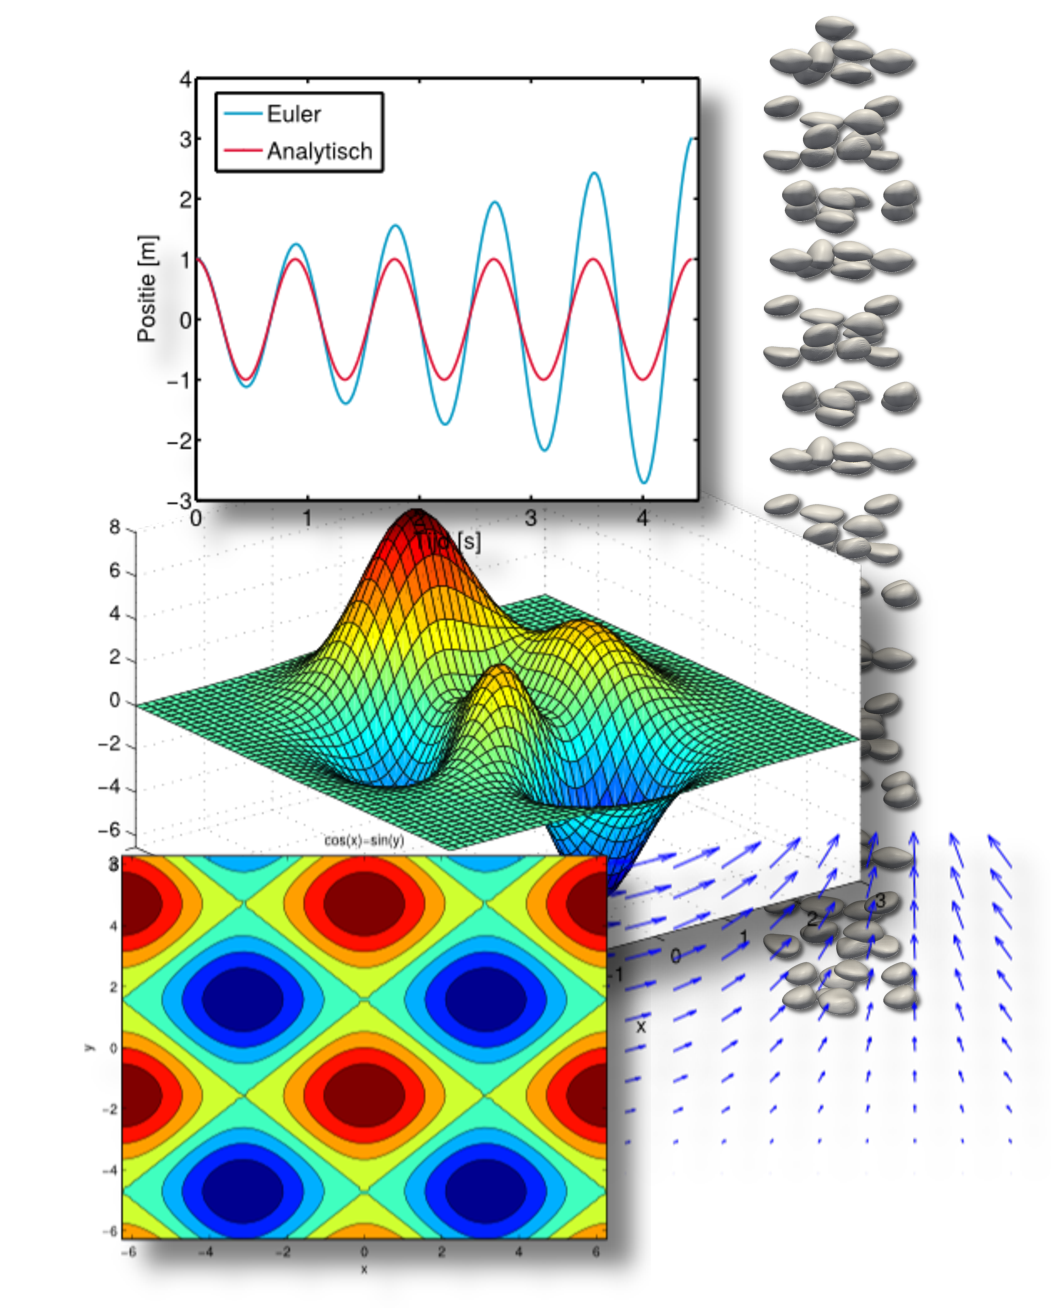
\includegraphics[width=\columnwidth]{visualisation}
 \end{columns}
\end{frame}

\begin{frame}[fragile]
  \frametitle{Plotting}
  \begin{lstlisting}
x = -5:0.1:5;
y = x.^2-4*x+3;
y2 = y + (2-4*rand(size(y))); (*@ \pause @*)
subplot(2,1,1); plot(x,y,'-',x,y2,'r.');
xlabel('X'); ylabel('Y'); title('Graph and Scatter'); (*@ \pause @*)
subplot(2,1,2); plot(x,abs(y-y2),'r-');
xlabel('X'); ylabel('Y'); title('Absolute error');
  \end{lstlisting}
  \centering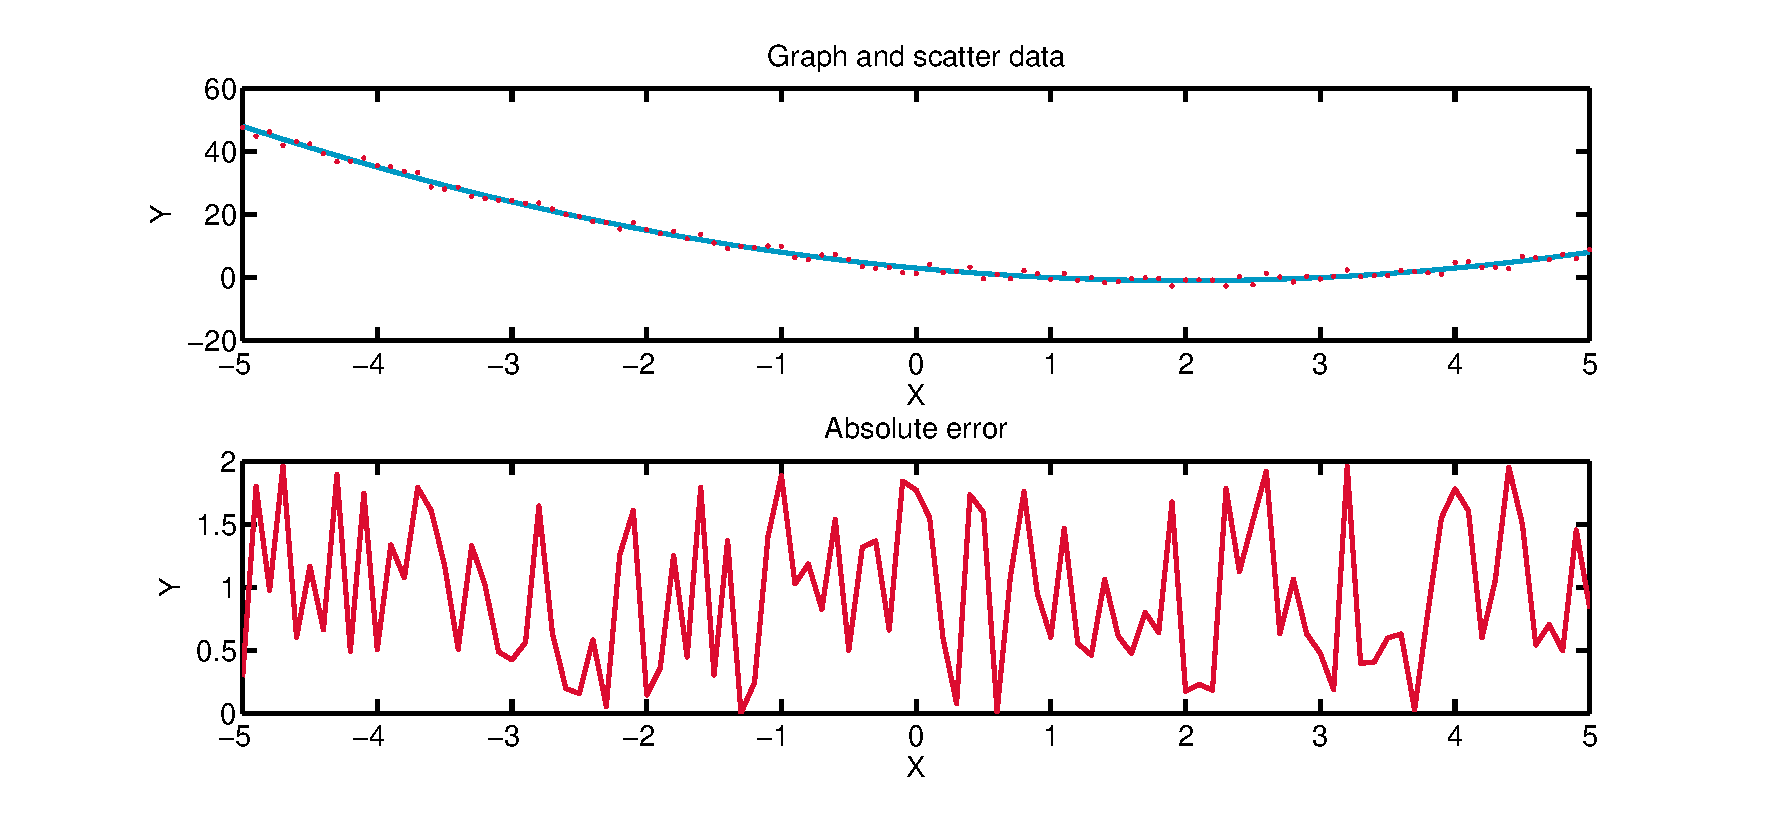
\includegraphics[width=0.8\textwidth]{showplot-utc}
\end{frame}

\begin{frame}[fragile]
  \frametitle{Plotting (2)}
  Easy plotting of functions can be done using the ezplot function: \lstinline$ezplot('x-sin(x)', [0 2*pi])$:
  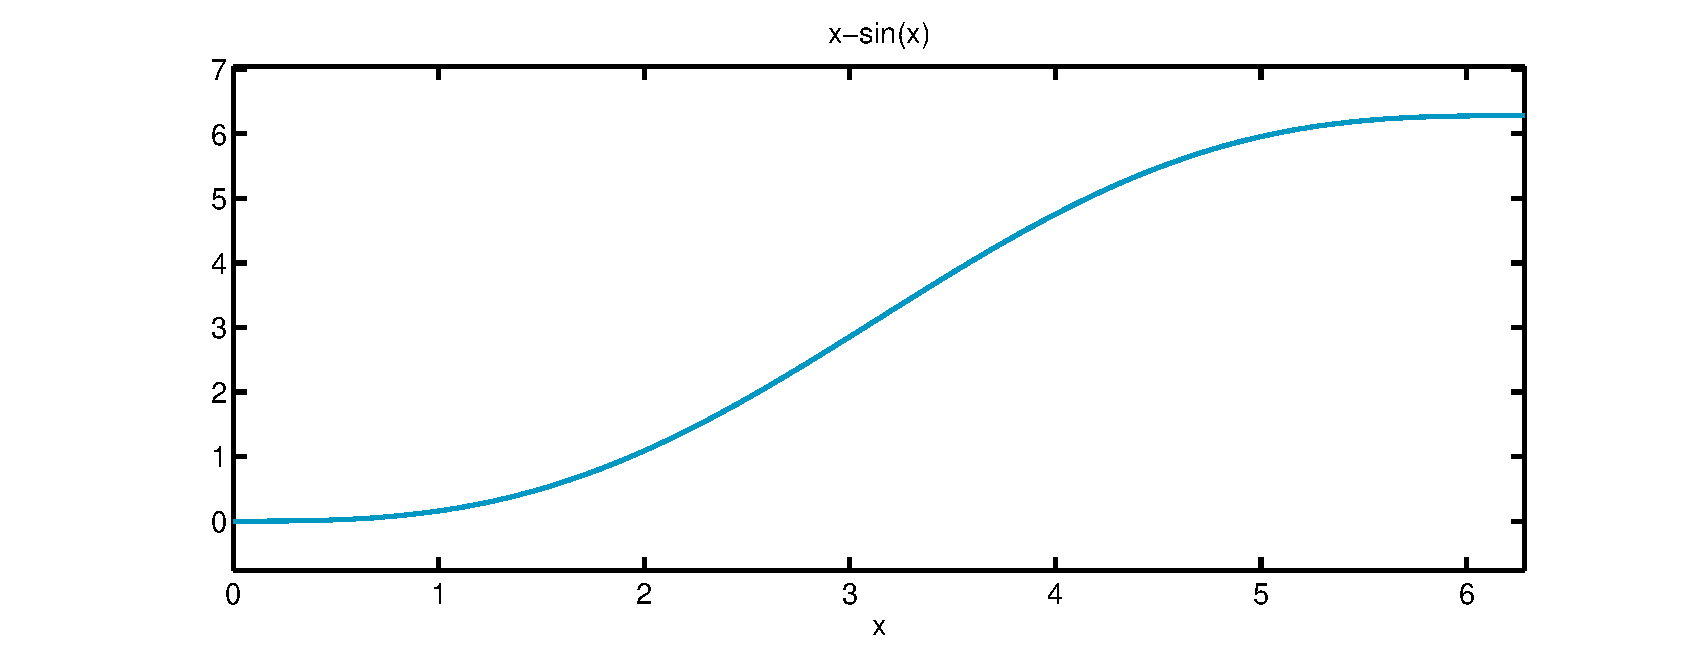
\includegraphics[width=0.7\textwidth]{show_ezplot-utc}\\
  Be careful with steep gradients: \lstinline$ezplot('x-sin(1/x)', [0 1])$% (use \lstinline$fplot$ instead)
  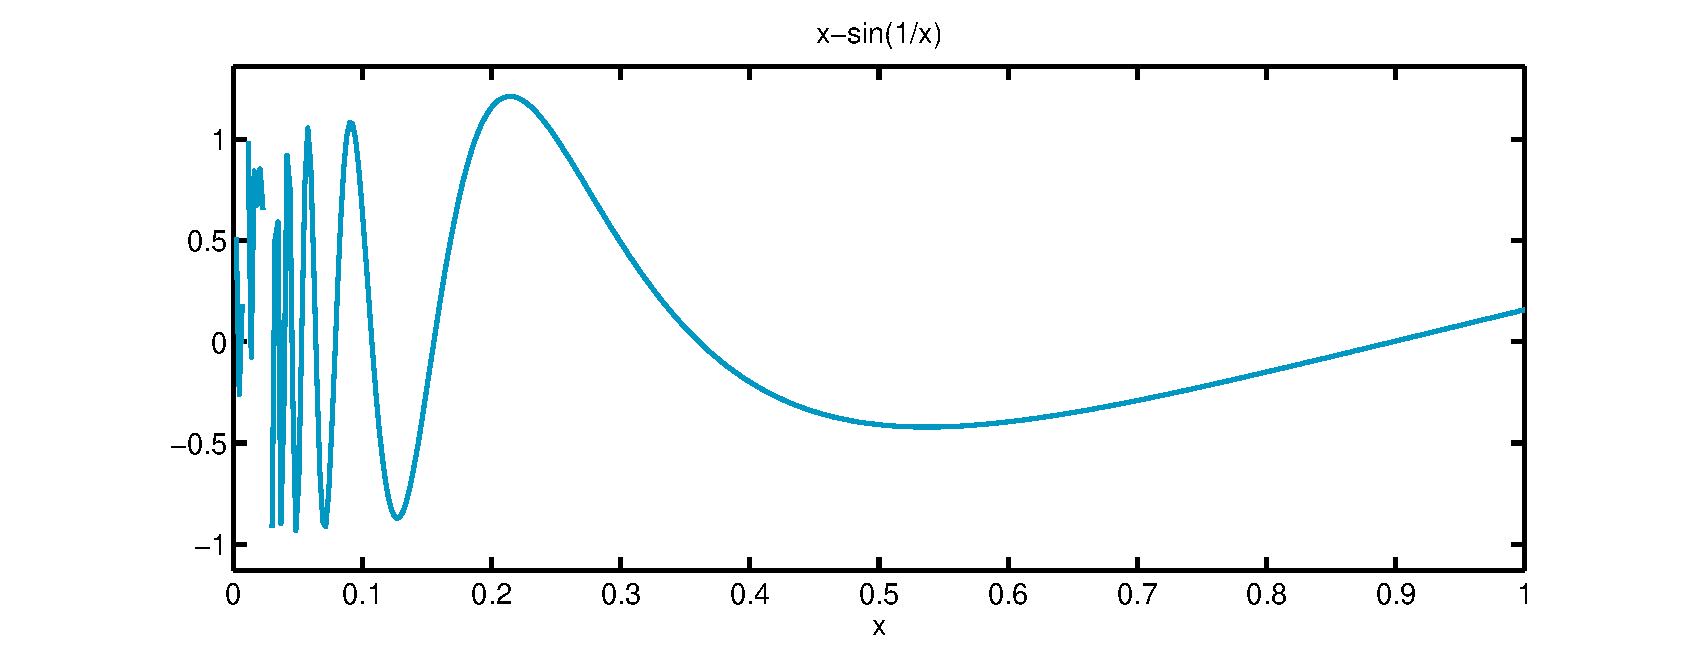
\includegraphics[width=0.7\textwidth]{show_ezplot2-utc}
\end{frame}

\begin{frame}[fragile]
  \frametitle{Other plotting tools}
  \begin{columns}
   \column{0.6\textwidth}
    \begin{itemize}[<+->]
      \item Errorbars: \lstinline$errorbar(x,y,err)$
      \item 3D-plots: \lstinline$plot3(x,y,z)$
      \item Histograms: \lstinline$histogram(x,20)$
%       \item Vectorplots: \lstinline$quiver(x,y,vx,vy)$
    \end{itemize}
   \column{0.4\textwidth}
    \includegraphics<1>[width=\columnwidth]{show_errorbar-utc}
    \includegraphics<2>[width=\columnwidth]{show_ezplot3-utc}
    \includegraphics<3>[width=\columnwidth]{show_hist-utc}
%     \includegraphics<3>[width=\columnwidth]{show_quiver-utc}
    
 \end{columns}
\end{frame}

\subsection*{Multi-dimensional data}
\begin{frame}[fragile]
  \frametitle{Multi-dimensional data}
  Matlab typically requires the definition of rectangular grid coordinates using \lstinline$meshgrid$:\\
  \begin{overlayarea}{\textwidth}{6cm}
  \begin{columns}[T]
   \column{0.6\textwidth}
    \begin{lstlisting}
[x y] = meshgrid(-2:0.1:2, -2:0.1:2);
z = x .* y .* exp(-x.^2 - y.^2);
    \end{lstlisting}
    \vskip1em
    \begin{itemize}
      \item<2-> Surface plot
      \item<3-> Contour plot
      \item<4-> Waterfall 
      \item<5> Ribbons
    \end{itemize}
   \column{0.4\textwidth}
   \begin{center}
      \includegraphics<2>[width=\columnwidth]{show_surf}
      \includegraphics<3>[width=\columnwidth]{show_contour}
      \includegraphics<4>[width=\columnwidth]{show_waterfall}
      \includegraphics<5>[width=\columnwidth]{show_ribbon}
   \end{center}
    \only<2>{
      \lstinline$surf(x,y,z);$
    }
    \only<3>{
      \lstinline$v=-0.5:0.05:0.5;$ \\
      \lstinline$contour(x,y,z,v,'ShowText', 'on');$
    }
    \only<4>{
    \lstinline$waterfall(x,y,z);$\\
    \lstinline$colormap(winter);$
    }
    \only<5>{
    \lstinline$ribbon(z);$
    }
 \end{columns}
 \end{overlayarea}
\end{frame}

\begin{frame}[fragile]
  \frametitle{Vector data}
  The gradient operator, as expected, is used to obtain the gradient of a scalar field. Colors can be used in the background to simultaneously plot field data:
  \begin{columns}[T]
   \column{0.6\textwidth}
    \begin{lstlisting}
[x y] = meshgrid(-2:0.2:2, -2:0.2:2);
z = x .* y .* exp(-x.^2 - y.^2)
[dx dy] = gradient(z,8,8)

% Background
contourf(x,y,z,30,'LineColor','none');
colormap(hot); colorbar;

axis tight; hold on;

% Vectors
quiver(x,y,dx,dy,'k');
    \end{lstlisting}
   \column{0.4\textwidth}
   \begin{center}
      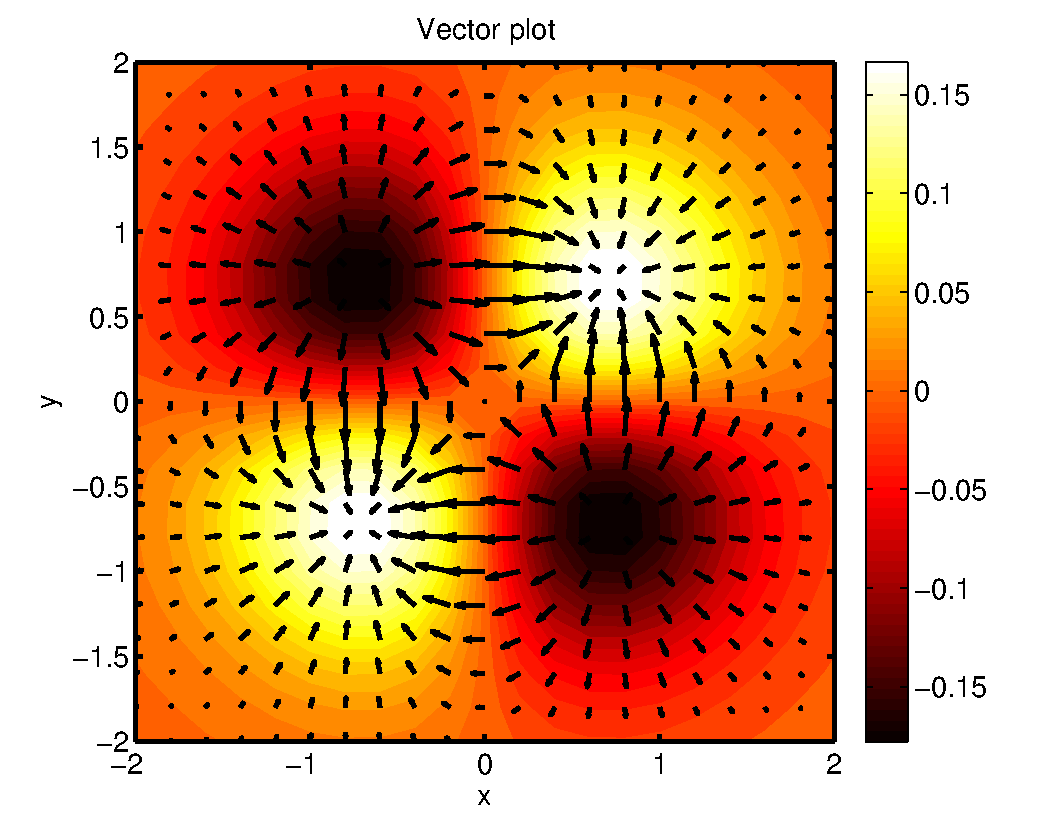
\includegraphics[width=\columnwidth]{show_vector}
    \end{center}
  \end{columns}
\end{frame}

\section{Functions: the sequel}
\againframe<2>{contents}
\subsection*{Function handles}
\begin{frame}[fragile]
  \frametitle{Functions: revisited}
  In MATLAB you can define your own functions to re-use certain functionalities. We now define the mathematical function $f = x^2+e^x$:
  \begin{lstlisting}
function y = f(x)
y = x.^2 + exp(x);
  \end{lstlisting}
  \pause
  Note:
  \begin{itemize}
    \item The first line of the file has to contain the \lstinline$function$ keyword
    \item The variables used are \emph{local}. They will not be available in your Workspace
    \item The file needs to be saved with the same name as the function, i.e. ``f.m''
    \item The semi-colon prevents that at each function evaluation output appears on the screen
    \item If \lstinline$x$ is an array, then \lstinline$y$ becomes an array of function values.
  \end{itemize}
\end{frame}

\begin{frame}[fragile]
  \frametitle{Anonymous functions}
  If you do not want to create a file, you can create an \emph{anonymous function}:
  \begin{lstlisting}
>> f = @(x) (x.^2+exp(x))
  \end{lstlisting}
  \pause
  \begin{itemize}
    \item \lstinline$f$: the name of the function
    \item \lstinline$@$: the function handle
    \item \lstinline$x$: the input argument
    \item \lstinline$x.^2+exp(x)$: the actual function
  \end{itemize}\pause
  \begin{lstlisting}
>> f(0:0.1:1)   
  \end{lstlisting}
\end{frame}

\begin{frame}[fragile]
  \frametitle{Using function handles}
  A function handle points to a function. It behaves as a variable
  \begin{lstlisting}
>> myFunctionHandle = @exp 
>> myFunctionHandle(1)
  \end{lstlisting}
  \pause
  Used a.o. for passing a function to another function, for instance for optimization functions.
  \[ f(x) = x^3 -x^2 -3\arctan{x}+1 \]
  \pause
  Matlab offers a function \lstinline$fzero$ that can find the roots of a function in a certain range:
  \begin{lstlisting}
>> f = @(x) x.^3 - x.^2 - 3*atan(x) + 1;
>> fzero(f,[-2 2])
>> ezplot(f)
>> f(ans)
  \end{lstlisting}
%   f
\end{frame}

\begin{frame}[fragile]
  \frametitle{Practice function handles}
  Consider the function
  \[ f(x) = -x^2 - 3x + 3 + e^{x^2} \]
  The built-in Matlab function \lstinline$fminbnd$ allows to find the minimum of a function in a certain range. Find the minimum of $f(x)$ on $-2\leq x \leq2$.
  Example usage:
  \begin{lstlisting}
x = fminbnd(fun,x1,x2)
  \end{lstlisting}
  \pause
  Answer using an anonymous function:
  \begin{lstlisting}
>> f = @(x) -x.^2 - 3*x + 3 + exp(x.^2)
>> ezplot(f,[-2 2])
>> fminbnd(f,-2,2)
>> f(ans)
  \end{lstlisting}
  \pause
  Various related functions are \lstinline$fzero$, \lstinline$feval$, \lstinline$fsolve$, \lstinline$fminsearch$. They will be discussed later in the course.
% 
%   fzero
%   feval
%   fsolve
%   fminsearch
%   f
\end{frame}


\section{Excel}
\againframe<2>{contents}
\subsection*{Solver and goal-seek}
\begin{frame}
  \frametitle{Solver and goal-seek}
  Excel comes with a goal-seek and solver function. For Excel 2010:
  \begin{itemize}
    \item Install via Excel $\Rightarrow$ File $\Rightarrow$ Options $\Rightarrow$ Add-Ins $\Rightarrow$ Go (at the bottom) $\Rightarrow$ Select solver add-in. You can now call the solver screen on the 'data' menu ('Oplosser' in Dutch)
    \item Select the goal-cell, and whether you want to minimize, maximize or set a certain value
    \item Enter the variable cells; Excel is going to change the values in these cells to get to the desired solution
    \item Specify the boundary conditions (e.g. to keep certain cells above zero)
    \item Click 'solve' (possibly after setting the advanced options). 
  \end{itemize}
\end{frame}

\begin{frame}
  \frametitle{Goal-seek: a simple example}
  Goal-Seek can be used to make the goal-cell to a specified value by changing another cell:
   \rowcolors[]{20}{white}{white}
   \renewcommand\arraystretch{1.25}
   \begin{itemize}
     \colorize<2> \item Open Excel and type the following:
    \begin{longtable}{|>{\columncolor{gray!40}}R{1cm}*{1}{|L{2cm}}*{1}{|L{4cm}}|}
    \hline
    \rowcolor{gray!40}& \centering A  & \centering B\tabularnewline
    \hline
    1 & x \hfill    & 3  \\
    \hline
    2 & f(x) \hfill & =--3*B1\textasciicircum2--5*B1+2  \\
    \hline
    3 &         & \\
    \hline
    \end{longtable}
    \colorize<3> \item Go to Data $\Rightarrow$ What-If Analysis $\Rightarrow$ Goal Seek...
    \begin{itemize}
      \colorize<3> \item Set cell: B2
      \colorize<3> \item To value: 0
      \colorize<3> \item By changing cell: B1
    \end{itemize}
    \colorize<4> \item OK. You find a solution of $0.333\ldots$.
   \end{itemize}
\end{frame}

\begin{frame}
  \frametitle{Solver: a simple example}
  The solver is used to change the value in a goal-cell, by changing the values in 1 or more other cells while keeping boundary conditions:
   \rowcolors[]{20}{white}{white}
   \renewcommand\arraystretch{1.25}
   \begin{itemize}
    \colorize<2> \item Use the following sheet:
    \begin{longtable}{|>{\columncolor{gray!40}}R{1cm}*{1}{|L{2cm}}*{1}{|L{2cm}}*{1}{|L{3cm}}|}
    \hline
    \rowcolor{gray!40}& \centering A  & \centering B& \centering C \tabularnewline
    \hline
    1 & & x & f(x)  \\
    \hline
    2 & x1 \hfill & 3 & =2*B2*B3--B3+2 \\
    \hline
    3 & x2 & 4& =2*B3--4*B2-4 \\
    \hline
    \end{longtable}
    \colorize<3> \item Go to Data $\Rightarrow$ Solver
    \begin{itemize}
      \colorize<3> \item Goalfunction: C2 (value of: 0)
      \colorize<3> \item Add boundary condition: C3 = 0
      \colorize<3> \item By changing cells: \$B\$2:\$B\$3 (you can just select the cells)
    \end{itemize}
    \colorize<4> \item Solve. You will find B2=0 and B3=2.
   \end{itemize}
\end{frame}

\begin{frame}
  \frametitle{Exercise}
  \rowcolors[]{1}{maincolor!20}{maincolor!10}
  \footnotesize\selectfont
  Use Excel functions to obtain the Antoine coefficients $A$, $B$ and $C$ for diethyl ether following the equation:
  \[
    \ln P = A - \frac{B}{T+C}
  \]
  $P$ in \si{\kilo\pascal}, $T$ in \si{\celsius}. Experimental data is given (see Canvas for the xls):
  \begin{columns}
  \column{0.35\textwidth}
    \begin{longtable}{c|r}
      $P$ [\si{\mmHg}]& $T$ [\si{\kelvin}] \\ \hline
      15.6   & 230.0\\
      29.1   & 239.3\\
      52.5   & 248.9\\
      91.9   & 258.9\\
      156.0  & 269.3\\
      257.6  & 280.1\\
      414.6  & 291.4\\
      651.1  & 303.1\\
      999.2  & 315.3\\
      1501.0 & 328.0\\ \hline
    \end{longtable}
  \column{0.65\textwidth}
  \pause
    \begin{enumerate}
      \item Dedicate three separate cells for $A$, $B$ and $C$. Give an initial guess of 15, 2800, 200.\pause
      \item Convert all values to proper units (hint: use e.g. =CONVERT(A2,``mmHg'',``Pa''))\pause
      \item Compute $P_\text{Antoine}$ (in \si{\pascal})\pause
      \item Compute $(P_\text{exp} - P_\text{Antoine})^2$, and sum this column\pause
      \item Start the solver, and aim for a value of 0 in the sum, by changing cells for $A$, $B$ and $C$.
    \end{enumerate}
  \end{columns}
\end{frame}

\section{Algorithms}
\subsection*{Introduction}
\againframe<2>{contents}
\begin{frame}[fragile]
  \frametitle{Algorithm design}
  \begin{enumerate}
    \colorize<1> \item \emph{Problem analysis}\\ Contextual understanding of the nature of the problem to be solved
    \colorize<2> \item \emph{Problem statement}\\ Develop a detailed statement of the mathematical problem to be solved with the program
    \colorize<3> \item \emph{Processing scheme}\\ Define the inputs and outputs of the program
    \colorize<4> \item \emph{Algorithm}\\ A step-by-step procedure of all actions to be taken by the program (\emph{pseudo-code})
    \colorize<5> \item \emph{Program the algorithm}\\ Convert the algorithm into a computer language, and debug until it runs
    \colorize<6> \item \emph{Evaluation}\\ Test all of the options and conduct a validation study
  \end{enumerate}
\end{frame}
% 
% \begin{frame}
%  \frametitle{Algorithm design}
%  \item Translate your problem to a formal procedure (recipe, pseudo-code)\pause
%    \begin{itemize}
%     \item What steps do I need to do? 
%     \item Can you break down a step further?
%     \item Is the order of the steps of importance?
%     \item Can I re-use certain parts? 
%   \end{itemize}
% \end{frame}

\subsection*{Example parabola}
\begin{frame}
  \frametitle{Example: finding the roots of a parabola}
  We are writing a program that finds for us the roots of a parabola. We use the form
  \[
    y = ax^2 + bx + c
  \]
  What is our program in pseudo-code? \pause
  \begin{enumerate}[<+->]
    \item Input data ($a$, $b$ and $c$)
    \item Identify special cases ($a=b=c=0$, $a=0$)
    \begin{description}
      \item[$a=b=c=0$] Solution indeterminate
      \item[$a=0$] Solution: $x = -\frac{c}{b}$
    \end{description}
    \item Find $D = b^2-4ac$
    \item Decide, based on $D$:
    \begin{description}
      \item[$D<0$] Display message: complex roots
      \item[$D=0$] Display 1 root value
      \item[$D>0$] Display 2 root values
    \end{description}
  \end{enumerate}
\end{frame}

\begin{frame}[plain,fragile]
  \frametitle{Example: finding the roots of a parabola}
  \small\selectfont
  \begin{lstlisting}[basicstyle=\scriptsize\ttfamily]
function x = parabola(a,b,c)
% Catch exception cases
if (a==0)
    if(b==0)
        if(c==0)
            disp('Solution indeterminate'); return;
        end
        disp('There is no solution');
    end
    x = -c/b;
end

D = b^2 - 4*a*c;
if (D<0)
    disp('Complex roots'); return;
    else if (D==0)
        x = -b/(2*a);
        else if (D>0)
                x(1) = (-b + sqrt(D))/(2*a);
                x(2) = (-b - sqrt(D))/(2*a);
                x = sort(x);
        end
    end
end
  \end{lstlisting}
\end{frame}


\begin{frame}[fragile]
  \frametitle{Example: finding the roots of a parabola}
  \begin{lstlisting}
>> roots([1 -4 -3])
ans =
    4.6458
   -0.6458
  \end{lstlisting}
\end{frame}
%
%\subsection*{Projectile}
%\begin{frame}[fragile]
%\scriptsize\selectfont
%  \frametitle{Example: projectile trajectory}
%  \begin{center}
%    \begin{tikzpicture}[scale=0.7,ball/.style={circle,minimum size=8mm,thick,shading=ball,ball color=maincolor,
%				      font=\sffamily\scriptsize},>=stealth',thick,node distance=0.75cm]
%      \node[ball,anchor=north] (ball) at (0,0) {$M$};
%      \node[anchor=north east] at (1.5,1.7) (aim) {};
%      \node[anchor=south east] at (aim.south) {$v_0$};
%      \uncover<2->{\node at (7.5,-0.5) (aim2) {};
%      \node[anchor=north] at (aim2) {Trajectory};}    
%      \node at (4,2.6) (aim3) {};
%      \uncover<3->{\node[ball,ball color=gray,fill opacity=0.5] (ball2) at (aim3) {};}
%      
%      \draw[->] (ball.north east) -> (aim.center);
%      \draw<2->[->,dashed] (ball.north east) parabola bend (aim3) (aim2);
%      \draw<3->[->] (ball2) -- node[midway,anchor=west]{$F_g=mg$} ($ (ball2)+(0,-2) $);
%    \end{tikzpicture}
%  \end{center}
%  \vskip1em
%  \begin{itemize}
%    \item<1-> A ball with mass $M$ is thrown at time $t = 0$ with a certain velocity $v(t) = v(0) = v_0$
%    \item<2-> We need to describe the trajectory of the ball over time
%    \item<3-> It is given that the only force acting on the ball is gravity: $F = Mg$
%  \end{itemize}
%\end{frame}
%
%\begin{frame}[fragile]
%\scriptsize\selectfont
%  \frametitle{Example: projectile trajectory}
%  Computers cannot solve a continuous equation; we need to \emph{discretize} the time into steps of size $\Delta t$. Create a time line:\\ \vskip2em\pause
%  \begin{tikzpicture}[snake=zigzag, line before snake = 5mm, line after snake = 5mm]
%    %draw horizontal line   
%    \draw (0,0) -- (6,0);
%    \draw[snake] (5.5,0) -- (8.5,0);
%    \draw (8,0) -- (10,0);
%
%    %draw vertical lines
%    \foreach \x in {0,2,4,6,8,10}
%      \draw (\x cm,3pt) -- (\x cm,-3pt);
%
%    %draw nodes
%    \draw (0,0) node[below=3pt] {$ t=0 $} node[above=3pt] {$ 1 $};
%    \draw (2,0) node[below=3pt] {$ \Delta t $} node[above=3pt] {$ 2 $};
%    \draw (4,0) node[below=3pt] {$ 2\Delta t $} node[above=3pt] {$ 3 $};
%    \draw (6,0) node[below=3pt] {$ 3\Delta t $} node[above=3pt] {$ 4 $};
%    \draw (8,0) node[below=3pt] {$ t_\mathrm{end}-\Delta t $} node[above=3pt] {$ n-1 $};
%    \draw (10,0) node[below=3pt] {$ t_\mathrm{end} $} node[above=3pt] {$ n $};
%    
%    \onslide<4>{
%      \draw (0,-1.5) node[above=1pt] {$x_0$};
%      \draw (0,-1.5) node[below=3pt] {$v_0$};
%    }
%    \onslide<5>{
%      \draw (0,-1.5) node[above=1pt] {$x(t)$};
%      \draw (0,-1.5) node[below=3pt] {$v(t)$};
%      \draw (2,-1.5) node[above=1pt] {$x(t+\Delta t)$};
%      \draw (2,-1.5) node[below=3pt] {$v(t+\Delta t)$};
%    }
%    \onslide<6>{
%      \draw (2,-1.5) node[above=1pt] {$x(t)$};
%      \draw (2,-1.5) node[below=3pt] {$v(t)$};
%      \draw (4,-1.5) node[above=1pt] {$x(t+\Delta t)$};
%      \draw (4,-1.5) node[below=3pt] {$v(t+\Delta t)$};
%    }
%    \onslide<7>{
%      \draw (4,-1.5) node[above=1pt] {$x(t)$};
%      \draw (4,-1.5) node[below=3pt] {$v(t)$};
%      \draw (6,-1.5) node[above=1pt] {$x(t+\Delta t)$};
%      \draw (6,-1.5) node[below=3pt] {$v(t+\Delta t)$};
%    }
%   \end{tikzpicture}
%\end{frame}
%
%\begin{frame}[fragile]
%\scriptsize\selectfont
%  \frametitle{Example: projectile trajectory}
%  \begin{itemize}
%    \item A Taylor expansion shows how the $x$-position is obtained at discrete time intervals: 
%    \[ f(x) = f(a) + \frac{f'(a)}{1!}(x-a) + \frac{f''(a)}{2!}(x-a)^2  + \ldots \]\pause
%    \[ x(t+\Delta t) = x(t) + \frac{\frac{dx}{dt}(t)}{1!}(t + \Delta t - t) + \frac{\frac{d^2x}{dt^2}}{2!}(t+\Delta t - t)^2  + O(\Delta t^3) \] \pause
%    \[ x(t+\Delta t) = x(t) + v(t)\Delta t + \frac{F}{2M}\Delta t^2  + O(\Delta t^3) \] \pause
%    \item Taking small time steps, we can discard $\Delta t^2$ and subsequent terms:
%    \[ x(t+\Delta t) = x(t) + v(t)\Delta t \] \pause
%    \item A similar approach is taken for the velocity:
%    \[ v(t+\Delta t) = v(t) + a(t)\Delta t \] \pause
%    \[ F = Ma \Rightarrow a = \frac{F}{M} \Rightarrow v(t+\Delta t) = v(t) + \frac{F(t)}{M}\Delta t \]
%  \end{itemize}
%\end{frame}
%
%\begin{frame}[fragile]
%\scriptsize\selectfont
%  \frametitle{Example: projectile trajectory}
%  Our mathematical model is as follows: \pause
%  \begin{enumerate}
%    \item Initialisation of parameters ($x_0$, $v_0$, $g$, $\Delta t$, $t_end$, $M$)\pause
%    \item Create storage vectors for time, position, velocity \pause
%    \item Start a time-marching loop \pause
%    \begin{itemize}
%    \scriptsize\selectfont
%      \item Calculate $x(t+\Delta t)$, then $F$, then $v(t+\Delta t)$:
%      \[ x(t+\Delta t) = x(t) + v(t)\Delta t \] 
%      \[ F = Mg \]
%      \[ v(t+\Delta t) = v(t) + \frac{F}{M}\Delta t \] \pause
%      \item Store current solution
%    \end{itemize}
%    \item Draw result and return solution vector $x$
%    \begin{itemize}
%      \item Exact solution:
%      \[
%        x(t) = x_0 + v_0 t + ( \frac{1}{2} -9.81 t^2 )
%      \]
%    \end{itemize}
%  \end{enumerate}
%\end{frame}
%
%\begin{frame}[fragile]
%  \frametitle{Example: projectile trajectory - solution (initialisation)}
%  \scriptsize\selectfont
%  \begin{lstlisting}
%function [pos,tim] = projectile(v0,M)
%
%% Initialise parameters
%t_end = 2;                  % End time
%deltat = 0.01;              % Time step
%x0 = 1;                     % Initial position
%
%nsteps = fix(t_end/deltat); % Number of time steps
%pos = zeros(nsteps,1);      % Position vector
%vel = zeros(nsteps,1);      % Velocity vector
%tim = zeros(nsteps,1);      % Time vector
%
%% Default values for mass and velocity
%if (nargin < 2)
%    M = 10;
%    if (nargin < 1)
%        v0 = 1;
%    end
%end
%  \end{lstlisting}
%\end{frame}
%
%\begin{frame}[fragile]
%  \frametitle{Example: projectile trajectory - solution (main program)}
%  \scriptsize\selectfont
%  \begin{lstlisting}
%pos(1) = x0;                % Store initial position
%vel(1) = v0;                % Store initial velocity
%
%% The time loop
%for n = 1:nsteps-1
%    pos(n+1) = position(pos(n),vel(n),deltat);
%    vel(n+1) = velocity(vel(n),M,deltat);
%    tim(n+1) = tim(n) + deltat;
%end
%
%% Plot results
%figure; plot(tim,pos, 'o');
%
%% Compare to analytical solution
%compareToExact(x0,v0,tim,pos);
%
%end
%  \end{lstlisting}
%\end{frame}
%
%\begin{frame}[fragile]
%  \frametitle{Example: projectile trajectory - solution (added functions)}
%  \scriptsize\selectfont
%  \begin{lstlisting}
%function F = force(M)
%% M:    mass of particle
%g = -9.81;
%F = M * g;
%end
%
%function v = velocity(vt,mass,dt)
%% vt:   velocity at previous time
%% mass: mass of particle
%% dt:   time step size
%v = vt + force(mass)/mass * dt;
%end
%
%function x = position(xt,vel,dt)
%% xt:   position at current time step
%% vel:  velocity at current time step
%% dt:   time step size
%x = xt + vel * dt;
%end
%  \end{lstlisting}
%\end{frame}
%
%\begin{frame}[fragile]
%  \frametitle{Example: projectile trajectory - solution (verification)}
%  \scriptsize\selectfont
%  \begin{lstlisting}
%function compareToExact(x0,v0,tim,pos)
%
%% Exact solution
%pos_ex = x0 + v0 * tim + ( 0.5 * -9.81 * tim .* tim );
%
%% Draw comparative figure
%figure;
%subplot(2,1,1)
%plot(tim,pos, 'o');
%hold on;
%plot(tim,pos_ex,'r-')
%subplot(2,1,2)
%stem(tim,pos_ex-pos,'r-')
%
%% Print the L2-error norm
%norm(pos_ex - pos)
%end
%  \end{lstlisting}
%\end{frame}
%
%\begin{frame}
%  \frametitle{Example: projectile trajectory - solution}
%  \begin{center}
%    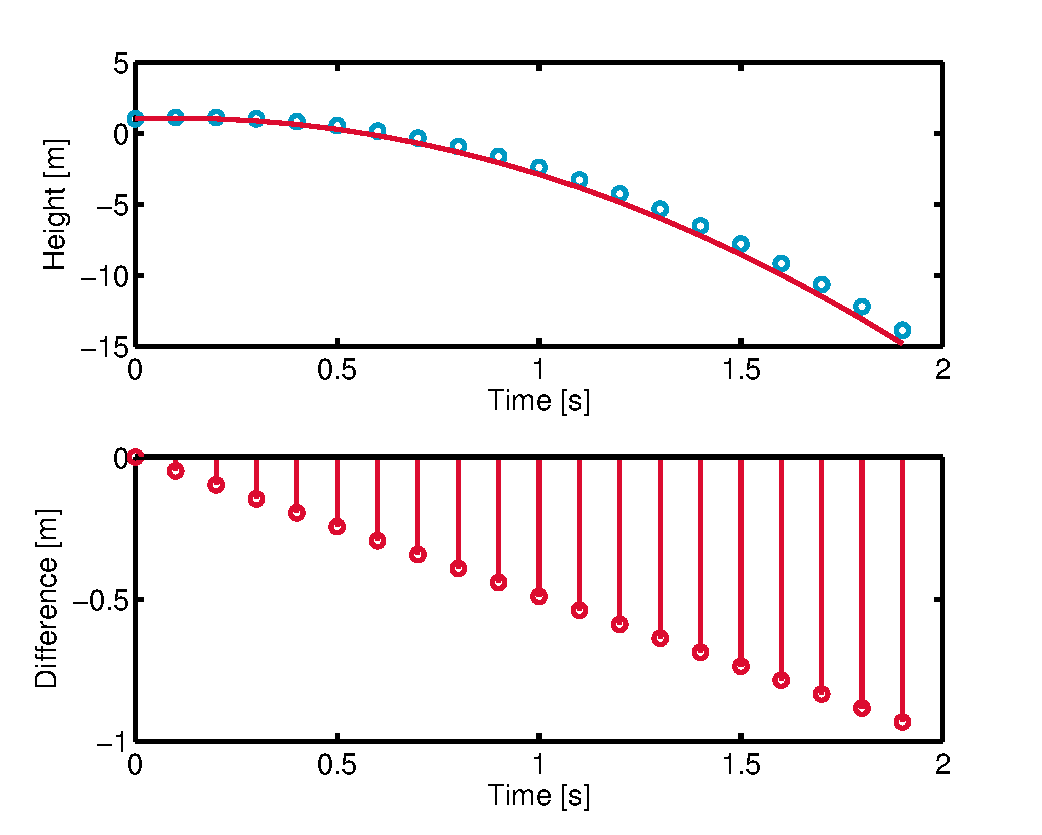
\includegraphics[width=0.8\textwidth]{projectile-utc}
%  \end{center}
%\end{frame}


\begin{frame}
 \frametitle{Advanced concepts}
 \begin{itemize}
   \item Object oriented programming: classes and objects
   \item Memory management: some programming languages require you to allocate computer memory yourself (e.g. for arrays)
   \item External libraries: in many cases, someone already built the general functionality you are looking for
   \item Compiling and scripting (``interpreted''); compiling means converting a program to computer-language before execution. Interpreted languages do this on the fly.
   \item Profiling, optimization, parallellization: Checking where your program spends the most of its time, optimizing (or parallellizing) that part.
 \end{itemize}\pause
    \only<beamer>{
      \tikzstyle{every picture}-=[remember picture]
      \begin{tikzpicture}[remember picture,overlay]{
	\node[xshift=0cm,yshift=0cm, anchor=center] at (current page.center) {
\includegraphics[width=\textwidth]{fullnerd2.png}};}
      \end{tikzpicture}}
\end{frame}


\section{Conclusions}
\subsection*{Conclusions}
\begin{frame}[fragile]
  \frametitle{In conclusion...}
  \begin{itemize}
    \colorize<1-> \item Algorithm design: define your problem, think ahead, make a scheme, sketch the interplay between variables and functions, then start programming
    \colorize<2-> \item Programming basics: variables, operators and functions, locality of variables, recursive operations
    \colorize<3-> \item Dealing with complex programs, verification of your algorithms, use of the debugger
    \colorize<4-> \item Visualisation: how to make 1D and 2D/3D plots, create a sensible and intuitive presentation of your data.
    \colorize<5-> \item Examples: a few practice cases
  \end{itemize}
\end{frame}

% \end{document}


% References
% http://ocw.mit.edu/courses/electrical-engineering-and-computer-science/6-00sc-introduction-to-computer-science-and-programming-spring-2011/unit-1/lecture-1-introduction-to-6.00/
% http://www.greenteapress.com/thinkpython/html/thinkpython002.html
% https://www.youtube.com/channel/UCLMQ21H2ad95faYG3yGCwYA
%http://stackoverflow.com/questions/4227145/in-matlab-are-variables-really-double-precision-by-default
%http://www.exploringbinary.com/why-0-point-1-does-not-exist-in-floating-point/

